\subsubsection{Algorithm Correctness}

We now prove the correctness of ${\tt OSR\_trans}$, showing that it yields strict OSR mappings if the applied rewrite rules satisfy the property that variables that are live at corresponding points in the original and rewritten program contain the same values. To characterize this property, we need to introduce some formal machinery based on bisimilarity of programs.

\begin{definition}[Program Bisimulation]
\label{de:bisimulation}
A relation $R\subseteq State\times State$ is a bisimulation relation between programs $\pi$ and $\pi'$ if for any input store $\sigma\in \Sigma$ it holds:
\begin{align*}
s\in\tau_{\pi\sigma} ~ & \wedge ~~ s'\in \tau_{\pi'\sigma} ~~ \wedge ~~ s~R~s' \Longrightarrow \\
1) & ~~ s\Rightarrow_{\pi} s_1 ~~~ \Longrightarrow ~~~ s'\Rightarrow_{\pi'} s'_1 ~~ \wedge  ~~ s_1~R~s'_1 \\
2) & ~~ s'\Rightarrow_{\pi'} s'_1 ~~~ \Longrightarrow ~~~ s\Rightarrow_{\pi} s_1 ~~ \wedge  ~~ s_1~R~s'_1
\end{align*}
\end{definition}

\noindent Notice that our notion of bisimulation between programs $\pi$ and $\pi'$ requires that $R$ be a bisimulation between transition systems $(\tau_{\pi\sigma}, \Rightarrow_{\pi})$ and $(\tau_{\pi'\sigma}, \Rightarrow_{\pi'})$ for any store $\sigma\in \Sigma$. %This implies that for any $\sigma$, $\tau_{\pi\sigma}$ is finite if and ony if $\tau_{\pi'\sigma}$ is finite; also, if they are finite, then they have the same length.

\begin{lemma}
\label{le:bisim-prop}
Let $R$ be a reflexive bisimulation relation between programs $\pi$ and $\pi'$. Then for any $\sigma\in \Sigma$ it holds:
\begin{equation}
\label{eq:bisim-prop-1}
|\tau_{\pi\sigma}|=|\tau_{\pi'\sigma}|
\end{equation}
\begin{equation}
\label{eq:bisim-prop-2}
\forall i\in dom(\tau_{\pi\sigma}), ~~ \tau_{\pi\sigma}[i]~R~\tau_{\pi'\sigma}[i]
\end{equation}
\end{lemma}

\begin{myproof}
We prove \eqref{eq:bisim-prop-2} by induction on $i$. The base follows from $\tau_{\pi\sigma}[0]=\tau_{\pi'\sigma}[0]=(\sigma,1)$ and the assumption that $R$ is reflexive. Assume as inductive hypothesis that $\tau_{\pi\sigma}[i]~R~\tau_{\pi'\sigma}[i]$ for any $i<|\tau_{\pi\sigma}|$. Since $|\tau_{\pi\sigma}|>i$ then $\tau_{\pi\sigma}[i] \Rightarrow_{\pi} \tau_{\pi\sigma}[i+1]$ by \ref{de:exec-trace}. It follows by \ref{de:bisimulation} that $\tau_{\pi\sigma}[i+1]~R~\tau_{\pi'\sigma}[i+1]$. 

To prove \eqref{eq:bisim-prop-1}, assume by contradiction that $|\tau_{\pi\sigma}|\neq|\tau_{\pi'\sigma}|$, e.g., $|\tau_{\pi\sigma}|>|\tau_{\pi'\sigma}|=k$. Since $|\tau_{\pi\sigma}|>k$ then $\tau_{\pi\sigma}[k]~R~\tau_{\pi'\sigma}[k]$ by \eqref{eq:bisim-prop-2} and $\tau_{\pi\sigma}[k] \Rightarrow_{\pi} \tau_{\pi\sigma}[k+1]$ by \ref{de:exec-trace}. It follows by \ref{de:bisimulation} that $\tau_{\pi'\sigma}[k] \Rightarrow_{\pi'} \tau_{\pi'\sigma}[k+1]$. Hence $|\tau_{\pi'\sigma}|>k$, contradicting the initial assumption. The proof for the case $|\tau_{\pi'\sigma}|>|\tau_{\pi\sigma}|$ is analogous.
\end{myproof}

\begin{definition}[Partial State Equivalence]
\label{de:state-equiv-relation}
For any function $A:\mathbb{N}\rightarrow 2^{Var}$, the {\em partial state equivalence} relation $R_A\subseteq State\times State$ is defined as:
\begin{equation*}
\begin{split}
R_A\triangleq\{ & (s, s')\in State\times State ~ | ~  \\
& s=(\sigma,l) ~ \wedge ~ s'=(\sigma',l) ~ \wedge ~ \sigma\vert_{A(l)} = \sigma'\vert_{A(l)} \}.
\end{split}
\end{equation*}
\end{definition}

\noindent Relation $R_A$ is clearly reflexive, symmetric, and transitive.

\begin{definition}[Live-Variable Bisimilar Programs]
\label{de:lvb-programs}
$\pi$ and $\pi'$ are {\em live-variable bisimilar} (LVB) if $R_{A}$ is a bisimulation relation between them, where $A=l\mapsto\live(\pi,l)\cap \live(\pi',l)$ is the function that yields for each program point $l$ the set of variables that are live at $l$ in both $\pi$ and $\pi'$.
\end{definition}

\noindent One consequence of \ref{de:state-equiv-relation}, which simplifies our formal discussion, is the following:

\begin{lemma}
\label{le:lvb-same-loc}
If $\pi$ and $\pi'$ are live-variable bisimilar, then for any $\sigma$, corresponding states in program traces $\tau_{\pi\sigma}$ and $\tau_{\pi'\sigma}$ are located at the same program points: $\forall i:$ $\tau_{\pi\sigma}[i]=(\sigma_i, l_i)$ $\wedge$ $\tau_{\pi'\sigma}[i]=(\sigma'_i, l'_i)$ $\Longrightarrow$ $l_i=l'_i$.
\end{lemma}
\begin{myproof}
Straightforward by \ref{le:bisim-prop} and \ref{de:state-equiv-relation}.
\end{myproof}

\begin{corollary}
If $\pi$ and $\pi'$ are live-variable bisimilar, then they have the same size: $\pi=\langle I_1,\ldots,I_n\rangle$ $\wedge$ $\pi'=\langle I'_1,\ldots,I'_{n'}\rangle$ $\Longrightarrow$ $n=n'$. 
\end{corollary}
\begin{myproof}
By \ref{le:bisim-prop}, \ref{le:lvb-same-loc}, and \eqref{eq:out-sem}, for any finite trace $\tau_{\pi\sigma}$ it holds $\tau_{\pi\sigma}[|\tau_{\pi\sigma}|]=(-,n+1)$ and $\tau_{\pi'\sigma}[|\tau_{\pi'\sigma}|]=(-,n+1)$. Hence both $\pi$ and $\pi'$ contain $n$ instructions.
\end{myproof}

\noindent We can now prove that \buildcomp\ generates correct OSR compensation code under the live-variable bisimilarity assumption. 

\begin{lemma}[Correctness of Algorithm \buildcomp]
\label{le:build-comp-corr}
Let $\pi$ and $\pi'$ be live-variable bisimilar programs. For each initial store $\sigma\in \Sigma$ it holds:
\begin{gather*}
\forall i\in dom(\tau_{\pi\sigma}): \chi\neq undef \implies \\
\mysem{\chi}(\sigma_i\vert_{\live(\pi,l_i)}) = \sigma'_i\vert_{\live(\pi',l_i)}
\end{gather*}
where $(\sigma_i,l_i)=\tau_{\pi\sigma}[i]$, $(\sigma'_i,l_i)=\tau_{\pi'\sigma}[i]$, and $\chi={\tt build\_comp}(\pi,l_i,\pi',l_i)$.
\end{lemma}

\begin{myproof}
The correctness of ${\tt build\_comp}$ relies on the ability of \reconstruct\ to produce compensation code for each variable that is live at OSR destination, but not at origin. Algorithm $\reconstruct(\wx, \pi, l, \pi', l', l'')$ aims to create a sequence of instructions that assigns \wx\ with the value that it would have assumed at $l''$ in $\pi'$, using as input the values of live variable at $l$ in $\pi$.

We proceed by induction on the recursive calls of \reconstruct. For the algorithm to succeed, there must be a unique definition {\tt x:=e} at some point $\hat{l}$ that dominates $l''$, otherwise $undef$ is thrown (see \myfigure\ref{fig:osr-reconstruct}). %If it is not unique, say there are two possible definitions {\tt x:=e} and {\tt x:=e'} that reach $l''$, then 
The base case happens when either:
\begin{enumerate}[itemsep=3pt, parsep=0pt]
 \item {\tt e} has no free variables (line 6), hence the compensation code for \wx\ is just {\tt x:=e} (line 9);
 \item the definition at $\hat{l}$ reaches both $l''$ and $l'$ (lines 1, 4) and \wx\ is live at both origin and destination (line 4), hence, since $\pi$ and $\pi'$ are live-variable bisimilar and \wx\ has the same value at $l$ and $l'$, then no compensation code for \wx\ is needed as the value of \wx\ at $l$ is the same that we would have had at $l''$;
 \item $\hat{l}$ has already been visited, so compensation code for \wx\ has already been created.
\end{enumerate}

\noindent Assume by inductive hypothesis that the recursive calls of \reconstruct\ have added to $\chi$ the code to assign each free variable $y$ of $e$ with the value they would have assumed at $\hat{l}$ (line 7). Then the value of \wx\ that we would have had at $\hat{l}$ is determined by \mytt{x:=e}, which is appended to $\chi$ (line 9).
\end{myproof}

\ifdefined\noauthorea
\begin{figure}[!ht]
\begin{center}
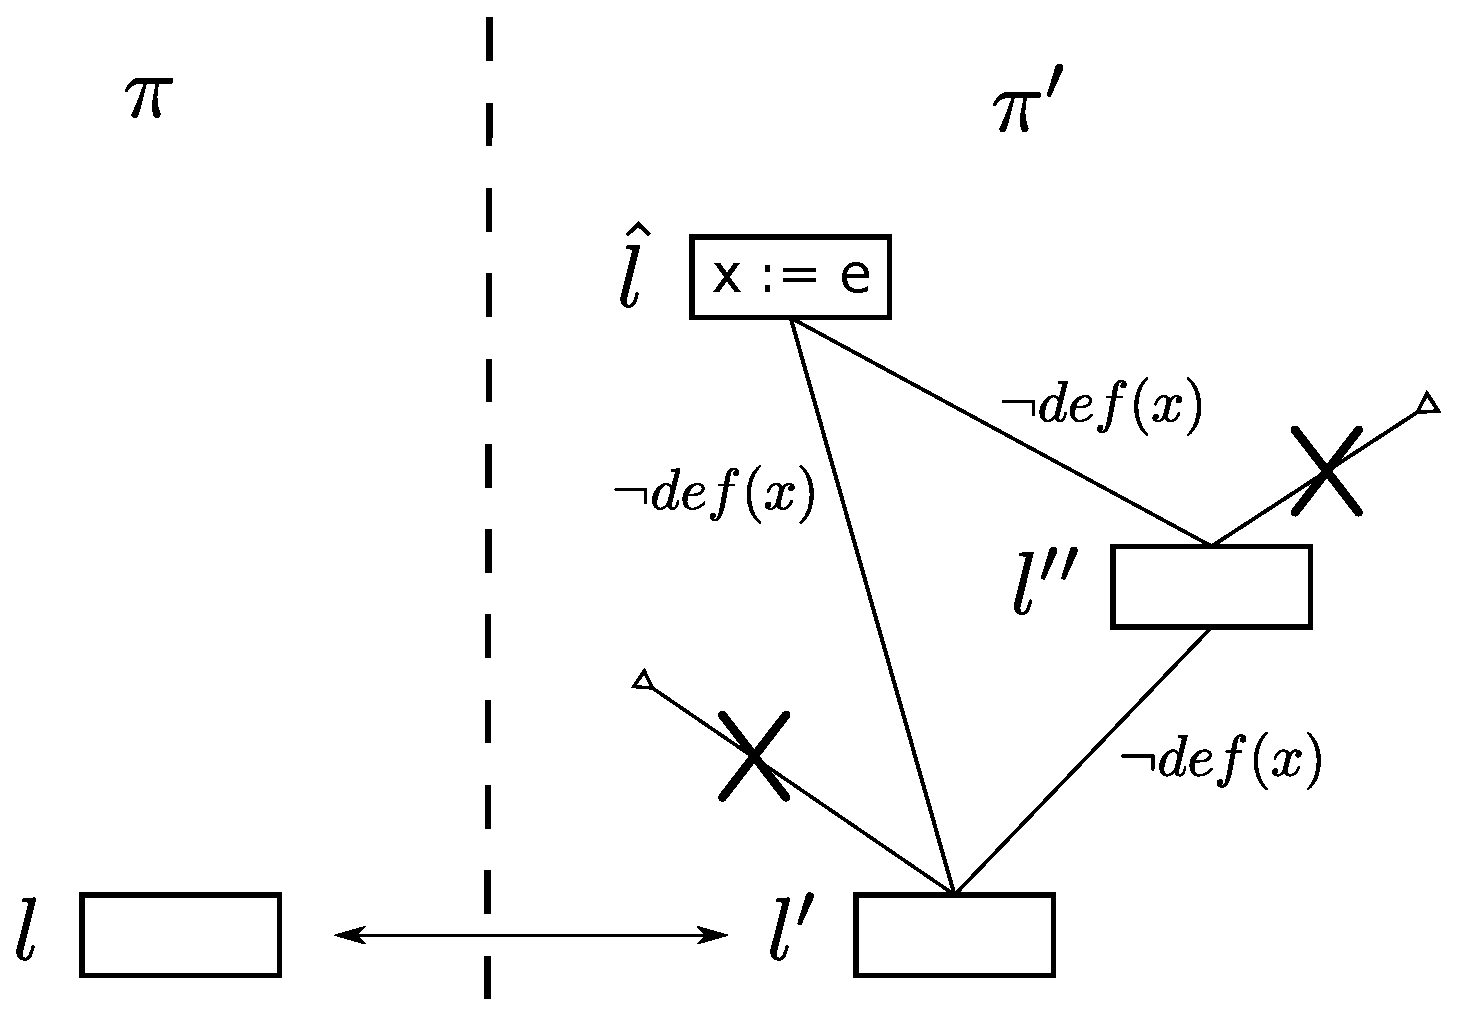
\includegraphics[width=0.49\textwidth]{figures/osr-reconstruct/osr-reconstruct.eps}
\caption{\protect\label{fig:osr-reconstruct} Algorithm \reconstruct\ identifies an assignment \mytt{x:=e} at $\hat{l}$ that reaches both $l'$ and $l''$, and no other definition of \wx\ is possible.}
\end{center}
\end{figure}
\fi

\begin{definition}[Live-Variable Equivalent Transformation]
\label{de:lve-trans}
A program transformation $T$ is {\em live-variable equivalent} (LVE) if for any program $\pi$, $\pi$ and $\mysem{T}(\pi)$ are live-variable bisimilar.
\end{definition}

\noindent We can finally establish the correctness of ${\tt OSR\_trans}$, which follows directly by \mylemma\ref{le:lvb-same-loc} and \mylemma\ref{le:build-comp-corr}:

\begin{theorem}
\label{th:osr-trans-correctness}
For any program $\pi$ and live-variable equivalent transformation $T$, if ${\tt apply}(\pi,T)\triangleq(\pi', \Delta_I, \Delta_I)$ where $\pi'=\mysem{T}(\pi)$ and $\Delta_I:[1,|\pi|]\rightarrow [1,|\pi|]$ is the identity mapping between program points, then ${\tt OSR\_trans}(\pi,T)$ $=(\pi',\mu_{\pi\pi'},\mu_{\pi'\pi})$ yields a strict OSR mapping $\mu_{\pi\pi'}$ between $\pi$ and $\pi'$ and a strict OSR mapping $\mu_{\pi'\pi}$ between $\pi'$ and $\pi$.
\end{theorem}

\paragraph*{Discussion.} We remark that the assumption of an identity mapping between program points, which is a necessary condition of live-variable bisimilarity, is without loss of generality as it can  always be enforced by padding programs with \wskip\ statements. For instance, the Hoist transformation of \myfigure\ref{fig:sample-trans}, which we prove to be LVE in \missing, replaces the hoisted instruction with a \wskip, and expects a \wskip\ to already exist at the point where it is moved. As we discuss in \missing, this is not required in a real compiler, as a transformation pass can be instrumented to capture code modifications that require updating the mapping.